\documentclass[11pt,a4paper]{scrartcl}
\usepackage[utf8]{inputenc}
\usepackage[english]{babel}
\usepackage{graphicx}
\usepackage{geometry}
\usepackage{fancyhdr}
\usepackage[table]{xcolor}
\usepackage{mathtools}
\usepackage{logicpuzzle}
\usepackage{listings}
\usepackage{hyperref}
\usepackage[toc,page]{appendix}
\hypersetup{
    colorlinks,
    citecolor=black,
    filecolor=black,
    linkcolor=black,
    urlcolor=black
}

 
\usepackage{fancyhdr} % Custom headers and footers
\pagestyle{fancyplain} % Makes all pages in the document conform to the custom headers and footers
\fancyhead{} % No page header - if you want one, create it in the same way as the footers below
\fancyfoot[L]{} % Empty left footer
\fancyfoot[C]{} % Empty center footer
\fancyfoot[R]{\thepage} % Page numbering for right footer
\renewcommand{\headrulewidth}{0pt} % Remove header underlines
\renewcommand{\footrulewidth}{0pt} % Remove footer underlines
\setlength{\headheight}{13.6pt} % Customize the height of the header
%
\lstset{ %
  basicstyle=\footnotesize,        % the size of the fonts that are used for the code
  breakatwhitespace=false,         % sets if automatic breaks should only happen at whitespace
  breaklines=true,                 % sets automatic line breaking
  captionpos=b,                    % sets the caption-position to bottom
  deletekeywords={...},            % if you want to delete keywords from the given language
  extendedchars=true,              % lets you use non-ASCII characters; for 8-bits encodings only, does not work with UTF-8
  frame=single,                    % adds a frame around the code
  keepspaces=true,                 % keeps spaces in text, useful for keeping indentation of code (possibly needs columns=flexible)
                keywordstyle=\color{blue},
                stringstyle=\color{red},
                commentstyle=\color{green},
                morecomment=[l][\color{magenta}]{\#},
  language=C,                 % the language of the code
  showspaces=false,                % show spaces everywhere adding particular underscores; it overrides 'showstringspaces'
  showstringspaces=false,          % underline spaces within strings only
  showtabs=false,                  % show tabs within strings adding particular underscores
  tabsize=4,                       % sets default tabsize to 2 spaces
}

\begin{document}
\lstset{language=Prolog,basicstyle=\footnotesize}
\renewcommand\lstlistingname{Code}
\DeclarePairedDelimiter{\ceil}{\lceil}{\rceil}
\definecolor{lgray}{gray}{0.65}
\definecolor{llgray}{gray}{0.90}

\newcommand{\horrule}[1]{\rule{\linewidth}{#1}} % Create horizontal rule command with 1 argument of height

\title{
\normalfont \normalsize
\textsc{KU Leuven} \\ [25pt] % Your university, school and/or department name(s)
\horrule{0.5pt} \\[0.4cm] % Thin top horizontal rule
\huge SORTES: DHCP Relay Agent \\ % The assignment title
\horrule{2pt} \\[0.5cm] % Thick bottom horizontal rule
}
 
\author{Bart Verhoeven \& Arne Van der Stappen} % Your name
 
\date{\normalsize December 31, 2014} % Today's date or a custom date
 
\maketitle % Print the title

\tableofcontents

\newpage

\section{User guide \label{sec:userguide}}
When the board is started up, it will act as a DHCP relay agent. More information about DHCP, and DHCP relay agents can be found on \href{http://en.wikipedia.org/wiki/Dynamic_Host_Configuration_Protocol} {\textbf{Wikipedia}}.

\subsection{Relay Agent configuration}
This relay agent has a static IP address (\textit{192.168.97.60/24}), and is configured to be able to work in the \textit{192.168.97.0/24} subnet. The relay agent itself is preconfigured and should work out of the box once the router and DHCP server are configured as below.

\subsection{DHCP Server configuration}
In order for this relay agent to work, the user needs to set up his own DHCP server. This server should be located in the \textit{192.168.96.0/24} subnet, with \textit{192.168.96.2/24} as ip address. These settings are hardcoded, and can be changed in Main.h if necessary. The server needs to be configured to be able to give out ip addresses in the subnet of the relay agent (\textit{192.168.97.60/24}). The relay agent will now relay DHCP messages from his subnet to the DHCP server.

\subsection{Router configuration}
The router between the two networks should have the NAT feature disabled.

\section{System Engineer guide}
\subsection{Compile}
To compile the program, simply type \textbf{\textit{make DHCPRelay}} while in the source root.

\subsection{Upload to Pic}
To upload the program to the pic, upload \textbf{\textit{main.hex}} using tftp as described in \href{http://www.foditic.org/SORTES\_14/missions/picUnixE.php}{\textbf{PIC development in C on UNIX howto}}.

\subsection{Tests}
To test the board, you can enable a DHCP client in the subnet of the DHCP relay agent. This client should now be assigned an IP address by the DHCP server.\\

The following tests have been run to confirm the correct working of the agent:
\begin{itemize}
\item A single PC connecting to the network and requesting a new IP
\item Multiple PC's connecting to the network at the same time and requesting a new IP
\item A PC with a static IP connecting to the network
\item A PC reconnecting to the network and requesting their old IP
\item A PC connected to the network for a longer period of time and renewing its lease
\end{itemize}

\section{Design Decisions}

The code of this relay agent was produced by translating ASG diagrams \ref{fig:asg} and \ref{fig:asgRelaying} to C.\\

As described in the ASG diagram, the relay agent starts out in a state where it initializes itself. In this initialization state interrupts and application specific hardware, the LCD, the timer, and the TCP/IP stack, are initialized. When this is completed, the agent will figure out the MAC address of its standard gateway (the router) through ARP. The agent will finally be in the Relaying state.\\

The relaying state consists of 4 components. These components are responsible for receiving and processing/sending messages to both client and server. Component 1 handles incoming client messages, component 2 processes and sends these messages to the server, component 3 receives server messages, and component 4 processes and sends these messages to the client.

\begin{figure}
	\centering
	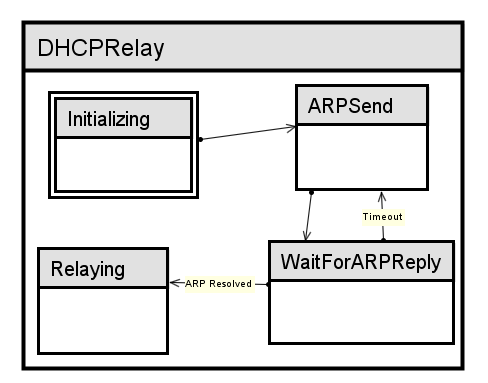
\includegraphics[width=1.0\textwidth]{../img/dhcprelay-asg.png}
	\caption{ASG diagram of the DHCP Relay Agent.\label{fig:asg}}
\end{figure}

\begin{figure}
	\centering
	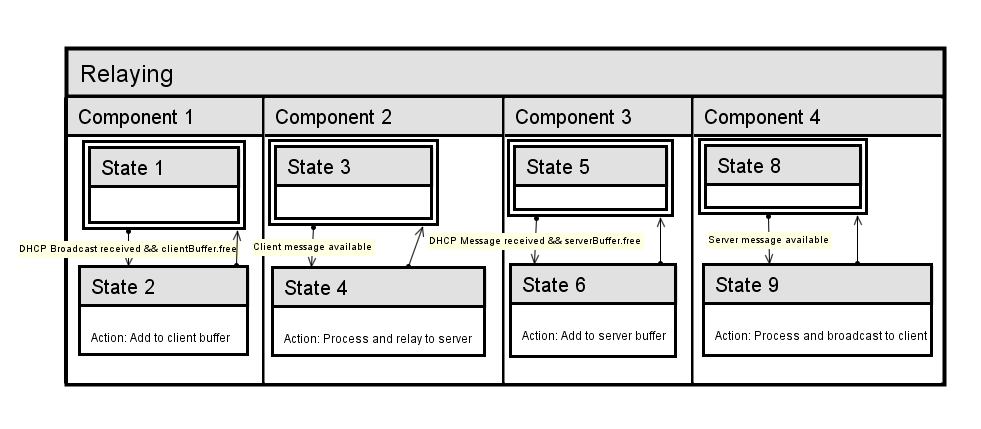
\includegraphics[width=1.0\textwidth]{../img/relaying-asg.png}
	\caption{ASG diagram of the Relaying state.\label{fig:asgRelaying}}
\end{figure}

\subsection{Seperate Client and Server components}
We have chosen to have seperate components dealing with broadcasts sent by clients (components 1 and 2) and replies sent by the server (components 3 and 4). These messages are already seperated because they arrive on different sockets. Because both types of messages are handled differently (the address for the relay is added in the messages that need to be send to the server, while messages to the client do not have to be altered) and they are sent out on different sockets as well, we have chosen to keep these seperate from start to end. For this, they also use seperate buffers: one for broadcasts received from clients and one for replies received from servers.\\
The given TCPIP Stack however only stores one UDP Packet at a time and as such there will never be a broadcast and a server reply at the same time. As a result, having seperate components does not give a performance advantage. However, we have decided to keep them seperate because they are logically different.

\subsection{Seperate Receive and Process/Send components}
For both broadcasts and serverreplies we also have seperate components for receiving and processing/sending. The Receive components (components 1 and 3) check if there is a message available on their respective socket and if so, they store this message in the appropriate buffer. The components will only check for new messages if there is room in the buffer.

The Process/Send components (components 2 and 4) will read messages from their buffers, do any required processing and then forward them on the appropriate relay.\\
The Process/Send component for client broadcasts (component 2) will add the IP of the Relay agent to the DHCP packet before forwarding it to the server.\\
The Process/Send component for server replies (component 4) will relay the received packet directly to clients via broadcast without any modification.

\subsection{Buffer size}
The internal buffers from which the processing-components of the application consume and for which the receiving-components of the application produce dhcp packages, have a size of one. This means that each pair of components (receiver-processor) of the application are tightly coupled. The consumer components have to consume the last packet before the producers can produce a new one. This limitation makes sure there is enough memory on the processor to hold the buffers. While this may seem like a heavy limitation, it is really not. The TCP/IP stack implementation provided will only put one message in the buffer at a time.\\
Given enough memory, this buffer could easily be extended to contain more than one message. This would not affect the workings of the components 

\subsection{Immeadiate state changes}

\newpage

\appendix
\section{Code}

\subsection{main.h}
\lstinputlisting[language=C]{../src/Main.h}

\subsection{main.c}
\lstinputlisting[language=C]{../src/Main.c}

\subsection{messageProcessor.h}
\lstinputlisting[language=C]{../src/messageProcessor.h}

\subsection{messageProcessor.c}
\lstinputlisting[language=C]{../src/messageProcessor.c}

\subsection{DHCPBuffer.h}
\lstinputlisting[language=C]{../src/DHCPBuffer.h}

\subsection{DHCPBuffer.c}
\lstinputlisting[language=C]{../src/DHCPBuffer.c}

\subsection{receiver.h}
\lstinputlisting[language=C]{../src/receiver.h}

\subsection{receiver.c}
\lstinputlisting[language=C]{../src/receiver.c}

\subsection{Debug.h}
\lstinputlisting[language=C]{../src/Debug.h}

\end{document}